\documentclass{vilniustech-en}
\vilniustechsetup{
    university={Vilnius Gediminas technical university},
    faculty={Faculty of Fundamental Sciences},
    cathedral={Department of Information Systems},
    workTitle={Software Defined Networks (SDNs) in Data Centers: pros, cons and risks},
    workType={Abstract},
    workAuthorName={Aurimas Šakalys},
    workAuthorGroup={ITSfm-22},
    workRecipient={prof. dr. Dalius Mažeika}
}
\addbibresource{bibliography.bib}
\VTDocumentBegin

\section{Operating model of physical networking devices}

At the very start of the development of physical networking devices, most of the actions performed by these devices were implemented using software. Most routers at the time were simple \textit{Unix} computers that would use software to search for entries within the routing table and forward the packets accordingly. On the \textit{datalink} layer, there were several competing products like \textit{IBMs Token Ring} and \textit{Ethernet}.

As time progressed and network sizes started increasing, so had the demand for fast switching for frames and routing of packets. Unfortunately performing this functionality purely within software was slower than desired. As such, some of the functionality of the devices started to be moved to implementations in hardware. First of such advancements came with specific circuits for quick hashing for table lookups, next \textit{content-addressable memory} technology emerged, which provided blazing fast lookups on destination addresses. 

\begin{wrapfigure}{l}{7cm}
\centering
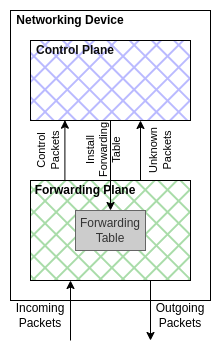
\includegraphics[width=5cm]{img/planes.drawio.png}
\caption{Planes of (most) physical networking devices}
\label{fig:planes}
\end{wrapfigure}    

Most of these devices had 2 (in some literature 3) logical abstraction layers called \textit{planes} (\autoref{fig:planes}):
\begin{itemize}
    \item Forwarding plane - it is responsible for receiving and transmitting packets, as well as execute forwarding decisions with the help of the forwarding table. If the forwarding plane encounters any control packets, or packets that the plane does not understand, they are forwarded towards the control plane to handle.
    \item Control plane - it is responsible for handling of control packets, unknown packets or packets without entry in the forwarding table.
\end{itemize}

The control plane, after a packet that have yet to been put into the forwarding table is forwarded to it, reads the packet, updates the forwarding table in the forwarding plane and sends the packet back. This way, the next time that a packet with the same destination is received, forwarding plane can handle it without the intervention of the control plane. 

Control plane is responsible for the control packets and these packets usually require to be processed by specific protocols, that are too complex to be implemented purely in hardware, as opposed to the forwarding plane, which has a possibility to be implemented purely in hardware.

In some literature, an additional management plane can be defined. Network managers interact and configures the device through this plane. This distinction could be simplified and the responsibilities of the management plane be merged with the control plane itself.

As mentioned previously, during the early days of networking, the forwarding plane had relatively simple hardware implementation and most of the complex work was delegated to the software implementation of the control plane. With the increase of network loads, complex handling within the control plane reduced the performance capability of the devices. With this, there was a need for moving of protocol handling and packet modifications to the forwarding plane arose. Here \textit{programmable rules} were introduced to the forwarding plane, which allowed for handling of some protocols to be moved away from the control plane. While more complex protocols would still have to be handled in the control plane, less complex ones were handled by the forwarding plane, allowing additional processing power to be freed in the control plane. 

\begin{wrapfigure}{r}{7cm}
\centering
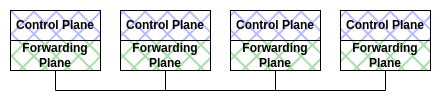
\includegraphics[width=7cm]{img/network_old.drawio.png}
\caption{Multiple connected dynamic network devices}
\label{fig:network_old}
\end{wrapfigure}  

Additionally, most of the protocols that are handled by the control plane pertains to the handling of topology update control protocols. This is due to the fact that these protocols were designed to provide stability within a large inter-network like the internet, where links between devices could go down often, devices would join and leave the topology and etc. Because of this, network devices are constantly bombarded with control packets, where they are trying to converge on valid forwarding table rules. 

While this is valid for devices in the internet, this might not be as attractive to networking devices within the data center. The network in the data center usually has a stable core topology and it does not change often. If the data center uses the type of networking devices that barrage everyone in the network with topology update packets, this type of traffic grows exponentially and takes up a very large portion of network traffic processing in the data center. Additionally, differently from the internet, both installation and removal of new hardware servers and creation and deletion of virtual machines within the data center happens only with approval of central orchestration software. As such, network devices that are capable of reacting to dynamic changes in the network do not seem to be up to the task, when in an environment of the data center.

\section{Software-defined network}

The inadequate operational model of dynamic networking devices in the data center gave rise to the idea of software-defined networking. The core idea is to remove the control plane from the networking devices and move it to one, centralized area (\autoref{fig:sdn_simple}).

\begin{wrapfigure}{l}{7cm}
\centering
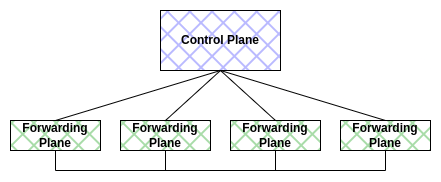
\includegraphics[width=7cm]{img/sdn_simple.drawio.png}
\caption{Simplified diagram of SDN}
\label{fig:sdn_simple}
\end{wrapfigure}  

The core benefit of this arrangement is that we remove most of the redundant topology update packets that were using up a significant portion of the resources in the network of the data center. Additionally, this would allow us to partially move the control to the central orchestrator, which in turn would allow the network to change quickly and accurately to reflect current status of hardware servers and virtual machines in the network.

\VTDocumentEnd